\addcontentsline{toc}{section}{Appendix}
\appendix
\counterwithin{figure}{section}
\counterwithin{lstlisting}{section}

\section{Implmentation of a discrete Kalman filter}\label{sec:KFimplementation}
The Kalman filter was implemented as a MATLAB S-function for use with Simulink.
\subsection*{kalman.m}
\lstinputlisting[label={lst:DiskKal}]{code/Part5/DiscKal.m}

\newpage
\section{Simulink Diagrams}\label{sec:simulink}
\begin{center}
	\centering
		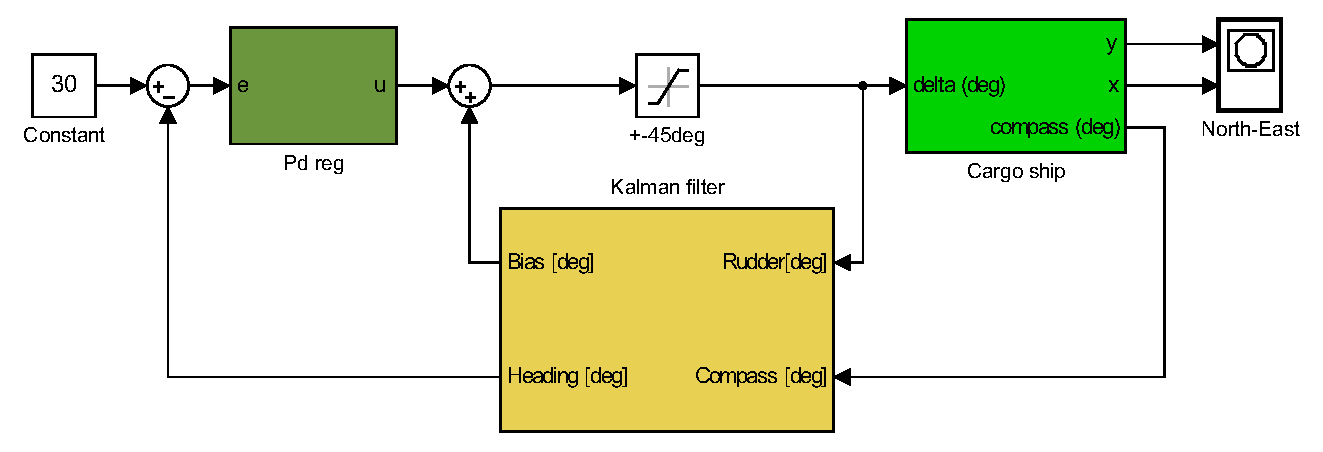
\includegraphics[width = \textwidth]{figures/simulink/sim_p5p5e_sim_p5p5e_sim.eps}
	\captionof{figure}{The complete system using the estimates from the Kalman filter.}
\label{fig:simulink_total}
\end{center}

\begin{center}
	\centering
		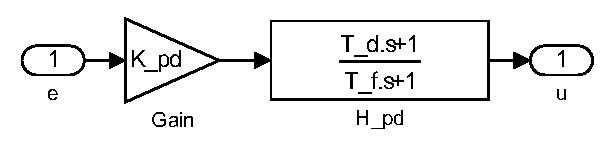
\includegraphics[width = \textwidth]{figures/simulink/sim_p5p5e_sim_pdreg.eps}
	\captionof{figure}{PD regulator.}
\label{fig:simulink_PD}
\end{center}

\begin{center}
	\centering
		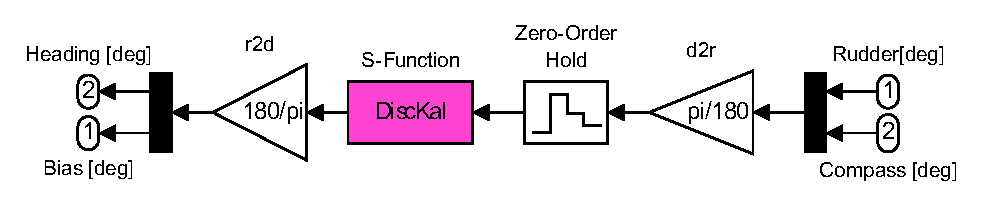
\includegraphics[width = \textwidth]{figures/simulink/sim_p5p5e_sim_kalmanfilter.eps}
	\captionof{figure}{Conversions and discrete Kalman filter s-function block.}
\label{fig:simulink_Kalman}
\end{center}